\documentclass[18pt,a4paper]{scrreprt}
\usepackage[utf8]{inputenc}
\usepackage[right=2cm,left=2cm,top=2cm]{geometry}
\usepackage{amsmath}
\usepackage{amsfonts}
\usepackage{amssymb}
\usepackage{listings}
\usepackage{color}
\usepackage{textcomp}
\definecolor{listinggray}{gray}{0.9}
\definecolor{lbcolor}{rgb}{0.9,0.9,0.9}
\usepackage{tikz}
\usetikzlibrary{automata,positioning}
\usetikzlibrary{arrows}
\usetikzlibrary{trees}
\tikzset{
  treenode/.style = {align=center, inner sep=0pt, text centered,
    },
  arn_n/.style = {treenode, circle, black,  draw=black,
    fill=white, text width=1.5em},% arbre rouge noir, noeud noir
}
\newcommand*\circled[1]{\tikz[baseline=(char.base)]{
            \node[shape=circle,draw,inner sep=1pt] (char) {#1};}}
%\author{kyriakosschwarz}
\title{Einfuehrung in die Theoretische Informatik}



%Math
\usepackage{amsmath}
\usepackage{amsfonts}
\usepackage{amssymb}
\usepackage{amsthm}
\usepackage{ulem}

\usepackage{amsmath}
\usepackage{graphicx}

%\usepackage{relsize}

%PageStyle
%\usepackage[ngerman]{babel} % deutsche Silbentrennung
\usepackage[utf8]{inputenc} 
\usepackage{fancyhdr, graphicx}

\usepackage{parskip}
\setlength{\textwidth}{17cm}
\setlength{\oddsidemargin}{-0.5cm}


% Shortcommands
\newcommand{\Bold}[1]{\textbf{#1}} %Boldface
\newcommand{\Kursiv}[1]{\textit{#1}} %Italic
\newcommand{\T}[1]{\text{#1}} %Textmode
\newcommand{\Nicht}[1]{\T{\sout{$ #1 $}}} %Streicht Shit durch

%Arrows
\newcommand{\lra}{\leftrightarrow} 
\newcommand{\ra}{\rightarrow}
\newcommand{\la}{\leftarrow}
\newcommand{\lral}{\longleftrightarrow}
\newcommand{\ral}{\longrightarrow}
\newcommand{\lal}{\longleftarrow}
\newcommand{\Lra}{\Leftrightarrow}
\newcommand{\Ra}{\Rightarrow}
\newcommand{\La}{\Leftarrow}
\newcommand{\Lral}{\Longleftrightarrow}
\newcommand{\Ral}{\Longrightarrow}
\newcommand{\Lal}{\Longleftarrow}

\newcommand{\ts}{\textsuperscript}

%Mine(new)
\newcommand{\tab}{\hspace*{2em}}
\newcommand{\cmark}{\ding{51}}%
\newcommand{\xmark}{\ding{55}}%

\usepackage{amssymb}% http://ctan.org/pkg/amssymb
\usepackage{pifont}% http://ctan.org/pkg/pifont

%Metadata
%\fancyfoot[C]{If you use this documentation for a exam, you should offer a beer to the authors!}
\title{
	\vspace{5cm}
	Einfuehrung in die Theoretische Informatik \\
}
\author{Kyriakos Schwarz,Roland Hediger}
\date{HS 2014}



\begin{document}

% Titelbild
\maketitle
\thispagestyle{fancy}
\newpage

% Inhaltsverzeichnis
%\pagenumbering{Roman}
\tableofcontents	  	
\newpage

%\setcounter{page}{1}
\pagenumbering{arabic}

% Inhalt Start

\chapter{Erste Woche}


\section{Sprachen}

Alphabet $\Sigma$: nichtleere endliche \uline{Menge} (von Zeichen)\\
\\
Wort ueber $\Sigma$: endliche \uline{Folge} von Zeichen aus $\Sigma$\\
\\
Leeres Wort: $\epsilon$ (epsilon)\\
\\
Menge aller Woerter ueber $\Sigma$: $\Sigma^*$\\
\\
\\
Konkatenation von Woertern $x,y$ ueber $\Sigma$:\\
\\
$x = x_1x_2 ... x_n$ \tab ,$x_i \in \Sigma$\\
$y = y_1y_2 ... y_n$\tab\:\: ,$y_i \in \Sigma$\\
\\
$x \cdot y = xy = x_1x_2 ... x_ny_1y_2 ... y_n$\\
\\
Java: $+$\tab\tab $""$ ($\epsilon$)\\
Haskell: $++$\tab $""$ ($\epsilon$)\\
\\
\\
\uline{Monoid}: Sei $M$ eine Menge und\\
\tab $\circ : M \times M \rightarrow^{total} M$ eine Verknuepfung\\
\\
Das Paar $(M, \circ)$ heisst ein \uline{Monoid}, falls gilt:\\
\\
1) $a \circ (b \circ c) = (a \circ b) \circ c$\tab ,$\forall a,b,c \in M$\\
\\
2) Es gibt ein $e \in M$ mit $a \circ e = a = e \circ a$\tab ,$\forall a \in M$\\
\\
$\qed$\\
\\
\\
\uline{Beispiel 1}\\
\\
$M = \Sigma^*, \circ = \cdot$\\
\\
$(\Sigma^*, \cdot)$ ist ein Monoid mit $\epsilon$ als neutralem Element\\
\\
$\qed$\\
\\
\uline{Beispiel 2}\\
\\
$\{\{ x =5; y = 6;\} z =7;\} \equiv \{x =5; \{y =6; z=7;\}\}$\\
\\
Komposition von Anweisungen assoziativ\\
\\
Neutrales Element: $;$ (Java) skip, NOP (no operation)\\
\\
$(x = 2*x; x = x+1;) \not\equiv (x = x+1; x = 2*x)$\\
\\
$\qed$\\
\\
\\
\uline{Sprache ueber $\Sigma$}:\\
\\
Menge von Woerter ueber $\Sigma$\\
\\
\uline{Beispiele}\\
\\
$\{\}$\tab 0 Woerter\\
$\{0,1,01,10\}$ Sprache uber $\Sigma = \{0,1\}$\\
$\Sigma^*$\\
$\{\epsilon\}$\tab 1 Wort\\
$\{\epsilon, 0, 00, 000, ...\}$ uber $\Sigma = \{0\}$\\
\\
\uline{Bem}\\
Sprache kann $\infty$ viele Woerter enthalten\\
Jedes Wort ist aber endlich\\
\\
\uline{Bem}\\
$\epsilon \in \Sigma^*$\\
$\Sigma^*$ immer $\infty$ gross\\
\\
\\
\uline{Operationen auf Sprachen}\\
\\
Seien $L_1$, $L_2$ Sprachen\\
\\
$L_1\cup L_2$ Vereinigungsmenge\\
\\
$L_1 \cdot L_2 = \{ xy \:\vert\: x \in L_1, y \in L_2\}$ (Kreuzprodukt)\\
\\
\\
Sei $(M, \circ)$ ein Monoid. Dann def.\\
\\
$a^0 = e$\tab\tab\:\:\:  ,$a \in M$\\
$a^n = a \circ a^{n-1}$\tab ,$n > 0$\\
\\
$\qed$\\
\\
\\
$L^0 = \{\epsilon\}$\\
\\
$L^n = L \cdot L^{n-1}$\tab ,$n>0$\\
\\
\\
\uline{Kleen' scher Stern}\\
\\
$L^* = L^0 \cup L^1 \cup L^2 \cup ...$\\
\\
\tab $= \{x_1, x_2, ..., x_k \:\vert\: k \geqslant 0, x_i \in L\}$\\
\\
\\
\uline{Aufgabe}\\
\\
$\Sigma = \{a,b,...,z\}$, $L_1 = \{good, bad\}$, $L_2 = \{cat, dog\}$\\
\\
$L_1 \cup L_2 = \{bad, cat, dog, good\}$\\
\\
$L_1 \cdot L_2 = \{goodcat, gooddog, badcat, baddog\}$\\
\\
$L_1^0 = \{\epsilon\}$\\
\\
$L_1^1 = \{good, bad\} = L_1 \cdot L_1^0 = L_1$\\
\\
$L_1^2  = \{goodgood, goodbad, badgood, badbad\}$\\
\\
$L_1^3 = \{ goodgoodgood, goodgoodbad, goodbadgood, goodbadbad,$\\
\tab\:\:\: $badgoodgood, badgoodbad, badbadgood, badbadbad\}$\\
\\
$L_1^* = L_1^0 \cup L_1^1 \cup L_1^2 \cup L_1^3 \cup ...$\\
\tab $= \{x_1, x_2, ..., x_k \:\vert k \geqslant 0, x_i \in, L_1\} = \{\epsilon, ...\}$\\
\\
$L_1 \cdot L_2 = \{goodcat, gooddog, badcat, baddog\} \neq L_2 \cdot L_1$\\
\\
$\vert M \vert =$ Anzahl Elemente von $M$\\ 
\\
\\
\rule{\textwidth}{0.4mm}\\
\section{Endliche Automaten DFA}

\uline{d}eterministic \uline{f}inite \uline{a}utomator\\
\\
\uline{Statisch}\\
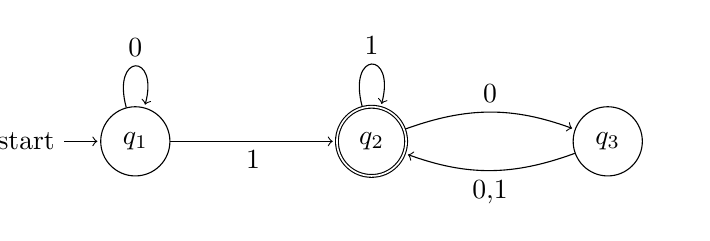
\begin{tikzpicture}[shorten >=1pt,node distance=3cm,on grid,auto] 
   \node[state,initial] (q_1)   {$q_1$}; 
%   \node[state] (q_1) [above right=of q_0] {$q_1$}; 
   \node[state, accepting] (q_2) [right=of q_1] {$q_2$}; 
   \node[state](q_3) [right=of q_2] {$q_3$};
    \path[->] 
%    (q_1) edge  node {0} (q_1)
%          edge  node [swap] {1} (q_2)
    (q_1) edge  node [swap] {1} (q_2)
          edge [loop above] node {0} ()
    (q_2) edge [bend left=20] node {0} (q_3)
          edge [loop above] node {1} ()      
    (q_3) edge [bend left=20] node {0,1} (q_2); 
%          edge [loop below] node {1} ();
\end{tikzpicture}
\\
\\
\uline{Dynamisch}\\
\\
\uline{Verarbeitung}\tab Input: $\xrightarrow{1101}$\\
\\
1. Start in $q_1$\tab Startzustand\\
2. Lese $\circled{1}101$\tab, $q_1 \rightarrow q_2$\\
3. Lese $1\circled{1}01$\tab, $q_2 \rightarrow q_2$\\
4. Lese $11\circled{0}1$\tab, $q_2 \rightarrow q_3$\\
5. Lese $110\circled{1}$\tab, $q_3 \rightarrow q_2$\\
6. Fertig $+$ akzeptiere, da $q_2$ akzeptierender Zustand ist und die Eingabe fertig gelesen ist.\\
\\
Liefert \uline{accept} oder \uline{fertig}\\
\\
\uline{Terminiert immer!}\\
\\
\\
\uline{Def}  \uline{DFA} : Ein DFA ist ein 5-Tupel $(Q, \Sigma, \delta, q_0, F)$ mit:\\
\\
1. $Q$ ist eine endliche nichtleere Menge von Zustaenden\\
\\
2. $\Sigma$ ist das \uline{Eingabealphabet} (z.B. $1101$)\\
\\
3. $\delta : Q \times \Sigma \rightarrow^{total} Q$\\
\tab \uline{Transitionsfunktion}\\
\\
4. $q_0$ Startzustand\\
\\
5. $F \subseteq Q$ Menge der akzeptierende Zustaende\\
\\
\\
\rule{\textwidth}{0.4mm}\\
\\
 
\chapter{Zweite Woche}


\section{DFA, NFA}


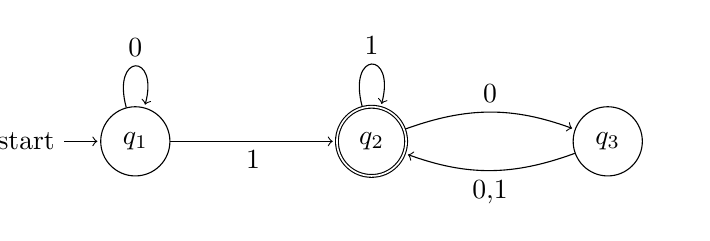
\begin{tikzpicture}[shorten >=1pt,node distance=3cm,on grid,auto] 
   \node[state,initial] (q_1)   {$q_1$}; 
   \node[state, accepting] (q_2) [right=of q_1] {$q_2$}; 
   \node[state](q_3) [right=of q_2] {$q_3$};
    \path[->] 
    (q_1) edge  node [swap] {1} (q_2)
          edge [loop above] node {0} ()
    (q_2) edge [bend left=20] node {0} (q_3)
          edge [loop above] node {1} ()      
    (q_3) edge [bend left=20] node {0,1} (q_2); 
\end{tikzpicture}
\\
\\
1. $Q = \{q_1, q_2, q_3\}$\\
\\
2. $\Sigma = \{0,1\}$\\
\\
3. $\delta : Q \times \Sigma \rightarrow Q$\\
\\
\tab $\delta(q_1, 0) = q_1$, $\delta(q_1, 1) = q_2$, ...\\
\\
4. $q_1$ Start\\
\\
5. $F = \{q_2\}$\\
\\
\\
\uline{Def Verarbeitung} (dynamisch)\\
\\
Sei $M = (Q, \Sigma, \delta, q_0, F)$ ein DFA\\
\\
Sei $w = x_1x_2x_3...x_m$ ein Wort ueber $\Sigma$ mit $x_i \in \Sigma$, $n \geqslant 0$ $[n=0 \rightarrow w = \epsilon]$\\
\\
\\
$M$ akzeptiert $w$, wenn eine Folge von Zustaenden existiert $r_0, r_1, r_2, ... , r_n$, mit:\\
\\
1. $r_0 = q_0$\\
2. $r_i = \delta(r_{i-1}, x_i), i \in \{1...m\}$\\
3. $r_n \in F$\\
\\
Sonst wird $w$ \uline{verworfen}\\
\\
\uline{accept} / \uline{reject}\\
\\
$\qed$\\
\\
\\
\rule{\textwidth}{0.4mm}\\
\\
\\
\begin{tabular}{|p{10cm}}
$M$ \uline{erkennt} Sprache $L$ falls\\
\\
$L = \{w \in \Sigma^{*} \:\vert\: M$ akzeptiert $w\}$\\
\end{tabular}
\\
\\
\\
\\
\begin{tabular}{|p{10cm}}
Eine Sprache heisst \uline{regulaer}, wenn ein\\
\\
\uline{DFA} existiert, der die Sprache erkennt\\ 
\end{tabular}
\\
\\
\\
\\
Automat $\rightarrow$ \uline{akzeptiert} / \uline{verwirft} \uline{Wort}\\
\tab $\searrow$\\
\tab \uline{erkennt} \uline{Sprache}\\
\tab\tab $\uparrow$\\
\tab \uline{recognise}
\\
\\
\rule{\textwidth}{0.4mm}\\
\\
$M_2:$ \tab $\Sigma = \{0,1\}$\\
\\
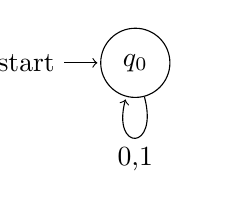
\begin{tikzpicture}[shorten >=1pt,node distance=3cm,on grid,auto] 
   \node[state,initial] (q_0)   {$q_0$}; 
    \path[->] 
    (q_0)  edge [loop below] node {0,1} (); 
\end{tikzpicture}
\\
\\
akzeptiert \uline{kein} Wort\\
\\
erkennt $\emptyset$\\
\\
\\
\rule{\textwidth}{0.4mm}\\
\\
$M_3:$ \tab $\Sigma = \{0,1\}$\\
\\
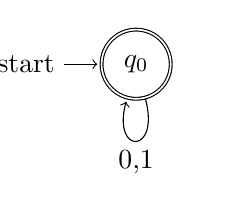
\begin{tikzpicture}[shorten >=1pt,node distance=3cm,on grid,auto] 
   \node[state,initial, accepting] (q_0)   {$q_0$}; 
    \path[->] 
    (q_0)  edge [loop below] node {0,1} (); 
\end{tikzpicture}
\\
\\
akzeptiert \uline{jedes} Wort\\
\\
erkennt $\Sigma^{*}$\\
\\
\\
\rule{\textwidth}{0.4mm}\\
\\
Zwei DFA heissen \uline{aequivalent}, wenn sie\\
dieselbe Sprachen erkennen\\
\\
\\
\uline{NFA}: nichtdeterministischer FA\\
\\
\\
$N_1:$ \tab $\Sigma = \{0,1\}$\\
\\
\\
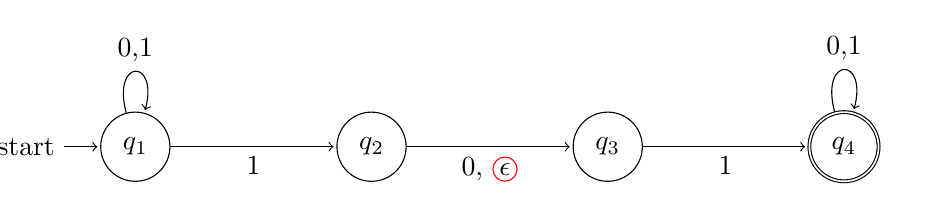
\begin{tikzpicture}[shorten >=1pt,node distance=3cm,on grid,auto] 
   \node[state,initial] (q_1)   {$q_1$}; 
%   \node[state] (q_1) [above right=of q_0] {$q_1$}; 
   \node[state] (q_2) [right=of q_1] {$q_2$}; 
   \node[state](q_3) [right=of q_2] {$q_3$};
   \node[state, accepting] (q_4) [right=of q_3] {$q_4$}; 
    \path[->] 
%    (q_1) edge  node {0} (q_1)
%          edge  node [swap] {1} (q_2)
    (q_1) edge  node [swap] {1} (q_2)
          edge [loop above] node {0,1} ()
    (q_2) edge node [swap] {0, \textcolor{red}{$\circled{\textcolor{black}{$\epsilon$}}$}} (q_3)
%          edge [loop above] node {1} ()      
    (q_3) edge node [swap] {1} (q_4) 
%          edge [loop below] node {1} ();
    (q_4) edge [loop above] node {0,1} ();
\end{tikzpicture}
\\
\\
Eingabe: $010110$\\
\\
\newpage
\textbf{Verarbeitung:}

\begin{tikzpicture}[->,>=stealth',level/.style={sibling distance = 15cm/#1,
  level distance = 2.5cm}]
\node [arn_n](Root) {$q_1$}   
child{node [arn_n] {$q_1$}
child{node [arn_n](q_1){$q_1$} 
	child {node [arn_n](q_10){$q_1$} 
		child{node [arn_n] (q_11) {$q_1$} 
			child{node [arn_n] (q_111) {$q_1$} 
				child{node [arn_n] (q_1110) [below = of q_111] {$q_1$} edge from parent node[right]{0}}		
			edge from parent node[left]{1}}
			child{node [arn_n] (q_1122) {$q_2$}
			child {node [arn_n] (q11220) [below = of q_1122] {$q_3$}edge from parent node[right]{0}}
			child {node [arn_n] (q_1123)[right= of q_1122]{$q_3$}
			edge from parent node[above]{$\epsilon$}}
			edge from parent node[left]{1}}	
			child{node [arn_n] (q_113) {$q_3$} edge from parent node[right]{1}}			
		edge from parent node[left]{1}}
		child{node [arn_n] (q_112) {$q_2$} 
			child{node [arn_n] (q_212) [right=of q_112] {$q_3$}
            child{ node [arn_n] {$q_4$} 
				child{ node [arn_n]{$q_4$} edge from parent node[right]{0}}            
            edge from parent node[right]{1}}			
			 edge from parent node[above]{$\epsilon$} }		
		edge from parent node[right]{1}}	
edge from parent node[left]{0}}
 edge from parent node[left] {1}
}
child{node [arn_n](q_2){$q_2$} 
	child{ node [arn_n](q_20)[below=of q_2] {$q_3$}
	child{ node [arn_n](q_41){$q_4$}
    	child{node [arn_n](q_411){$q_4$}
			child{node [arn_n] (q_4111){$q_4$} edge from parent node[right]{0}}    	
    	 edge from parent node[right]{1}}	
	 edge from parent node[right]{1}}	
	 edge from parent node[right]{0}}
	child{ node [arn_n](q_3) [right=of q_2] {$q_3$} edge from parent node[above]{$\epsilon$}}edge from parent node[right]{1}} edge from parent node[left] {0}}
;
%Extra todo :http://tex.stackexchange.com/questions/63612/tikz-tree-drawing-with-comments-to-each-level
\end{tikzpicture}
\\
\\
\rule{\textwidth}{0.4mm}\\
\newpage

%\begin{tabular}{|p{10cm}}
\uline{Def:} \: $P = P(Q) = 2^Q =$ \uline{Potenzmenge} \\
ist Menge aller Teilmengen von $Q$ \\
\\
$\Sigma_{\epsilon} = \Sigma \cup \{\epsilon\}$\\
%\end{tabular}
\\
\\
\\
\\
\uline{Def}  \uline{DFA} : Ein NFA ist ein 5-Tupel $(Q, \Sigma, \delta, q_0, F)$ mit:\\
\\
1. $Q$ ist eine endliche nichtleere Menge von Zustaenden\\
\\
2. $\Sigma$ ist das \uline{Eingabealphabet} (z.B. $1101$)\\
\\
3. $\delta : Q \times \Sigma_{\textcolor{red}{\epsilon}} \rightarrow^{total} P(Q)$\\
\tab \uline{Transitionsfunktion}\\
\\
4. $q_0 \in Q$ Startzustand\\
\\
5. $F \subseteq Q$ Menge der akzeptierende Zustaende\\
\\
\\
\rule{\textwidth}{0.4mm}\\
\\

\chapter{Dritte Woche}


\section{NFA}

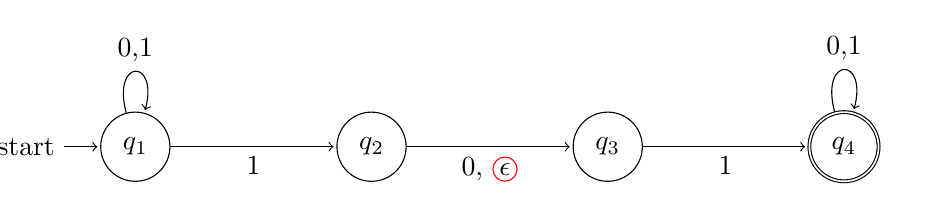
\begin{tikzpicture}[shorten >=1pt,node distance=3cm,on grid,auto] 
   \node[state,initial] (q_1)   {$q_1$}; 
%   \node[state] (q_1) [above right=of q_0] {$q_1$}; 
   \node[state] (q_2) [right=of q_1] {$q_2$}; 
   \node[state](q_3) [right=of q_2] {$q_3$};
   \node[state, accepting] (q_4) [right=of q_3] {$q_4$}; 
    \path[->] 
%    (q_1) edge  node {0} (q_1)
%          edge  node [swap] {1} (q_2)
    (q_1) edge  node [swap] {1} (q_2)
          edge [loop above] node {0,1} ()
    (q_2) edge node [swap] {0, \textcolor{red}{$\circled{\textcolor{black}{$\epsilon$}}$}} (q_3)
%          edge [loop above] node {1} ()      
    (q_3) edge node [swap] {1} (q_4) 
%          edge [loop below] node {1} ();
    (q_4) edge [loop above] node {0,1} ();
\end{tikzpicture}
\\
\\
\uline{Berechnung NFA}\\
\\
Sei $N = (Q, \Sigma, \delta, q_0, F)$ ein NFA\\
\\
Sei $w = y_1y_2...y_m$, $y_i \in \Sigma{\epsilon}$\\
\\
Es existiere eine Folge von Zustaenden\\
$r_0r_1r_2...r_m$, $r_i \in Q$ mit\\
\\
1. $r_0 = q_0$\\
2. $r_i \in \delta(r_{i-1}, y_i)$, $1 \leqslant i \leqslant m$\\
3. $r_m \in F$\\
\\
Dann \uline{akzeptiert} $N$ das Wort $w$, sonst \uline{verwirft} es\\
\\
$\qed$\\
\\
\\
\uline{Beispiel} \tab $N_1$ auf $010110$ (unseres Beispiel)\\
\\
1\ts{er} Weg\\ \tab $q_1$ \tab $q_1$ \tab $q_2$ \tab $q_3$ \tab $q_4$ \tab $q_4$ \tab $q_4$\\
\tab\tab 0 \tab 1 \tab\:\: 0 \tab 1 \tab\:\: 1 \tab 0\\
\\
2\ts{er} Weg\\ \tab $q_1$ \tab $q_1$ \tab $q_1$ \tab $q_1$ \tab $q_2$ \tab $q_3$ \tab $q_4$ \tab $q_4$\\
\tab\tab 0 \tab 1 \tab\:\: 0 \tab 1 \tab\: \textcolor{red}{$\circled{\textcolor{black}{$\epsilon$}}$} \tab 1 \tab\:\: 1\\
\\
\\
\rule{\textwidth}{0.4mm}\\
\\
\uline{Theorem}: Jeder NFA hat einen aequivalenten DFA $\qed$\\
\\
\uline{Beweis}: Sei $N = (Q, \Sigma, \delta, q_0, F)$ ein NFA der $L$ erkennt\\
Wir \uline{konstruieren} ein DFA $D = (Q', \Sigma', \delta', q_0', F')$, der ebenfalls $L$ erkennt\\
\\
1. $Q' = 2^Q = P(Q)$\\
\\
2. $\delta'(R,\alpha) = \underset{r \in R}{\scalebox{1.5}{$\cup$}}{\delta(r,\alpha)}$\\
\tab\: $\uparrow $\\
\tab \scalebox{0.8}{$\in Q'$}\\
\\
\\
Sei $E(R) = \{ q \in Q \:\vert\: q$ kann von $R$ aus durch $\epsilon$-Trans erreicht werden$\}$\\
\\
3. $q_0' = E(\{q_0\})$\\
\\
4. $F' = \{ R \in Q' \:\vert\: R \cap F \neq \emptyset \}$\\
\\
$\qed$\\
\\
\\
\rule{\textwidth}{0.4mm}\\
\\
\uline{Uebung}\\

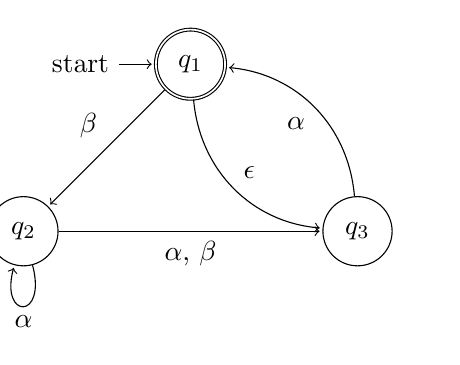
\begin{tikzpicture}[shorten >=1pt,node distance=3cm,on grid,auto] 
   \node[state,initial, accepting] (q_1)   {$q_1$}; 
   \node[state] (q_2) [below left=of q_1] {$q_2$}; 
   \node[state] (q_3) [below right=of q_1] {$q_3$}; 
   %\node[state,accepting](q_3) [below right=of q_1] {$q_3$};
    \path[->] 
    (q_1) edge  node [swap] {$\beta$} (q_2)
          edge [bend right=40] node {$\epsilon$} (q_3)
    (q_2) edge  node [swap]  {$\alpha$, $\beta$} (q_3)
          edge [loop below] node {$\alpha$} ()
    (q_3) edge [bend right=40] node {$\alpha$} (q_1); 
\end{tikzpicture} 
\\
\\
$Q = \{q_1,q_2,q_3\}$\\
$\Sigma = \{\alpha, \beta\}$\\
$\delta = \{ \delta(q_1,\beta) = q_2$,\\
\tab\: $\delta(q_1,\epsilon) = q_3$\\
\tab\: $\delta(q_2,\alpha) = q_2$\\
\tab\: $\delta(q_2,\alpha) = q_3$\\
\tab\: $\delta(q_2,\beta) = q_3$\\
\tab\: $\delta(q_3,\alpha) = q_1 \}$\\
$q_0 = q_1$\\
$F = \{q_1\}$\\
\\
\\
$\rightarrow$ DFA\\
\\
1. $Q' = P(Q) = \{\{\}, \{q_1\}, \{q_2\}, \{q_3\}, \{q_1,q_2\},$\\
\tab \tab \tab \tab $\{q_1,q_3\}, \{q_2,q_3\}, \{q_1,q_2,q_3\}\}$\\
\\
2. $\delta'$: \\
\begin{tabular}{ l | l | l }                       
   & $\alpha$ & $\beta$ \\
  \hline
  $\{\}$ & $\{\}$ & $\{\}$ \\
  $\{q_1\}$ & $\{\}$ & $\{q_2\}$ \\
  $\{q_2\}$ & $\{q_2,q_3\}$ & $\{q_3\}$ \\
  $\{q_3\}$ & $\{q_1,q_3\}$ & $\{\}$ \\
  $\{q_1,q_2\}$ & $\{q_2,q_3\}$ & $\{q_2,q_3\}$ \\
  $\{q_1,q_3\}$ & $\{q_1,q_3\}$ & $\{q_2\}$ \\
  $\{q_2,q_3\}$ & $\{q_1,q_2,q_3\}$ & $\{q_3\}$ \\
  $\{q_1,q_2,q_3\}$ & $\{q_1,q_2,q_3\}$ & $\{q_2,q_3\}$ \\
\end{tabular}
\\
\\
\\
3. $q_0' = E(\{q_0\}) = E(\{q_1\}) = \{q_1,q_3\}$\\
\\
4. $F' = \{\{q_1\}, \{q_1,q_2\}, \{q_1, q_3\}, \{q_1, q_2, q_3\}\}$\\
\\
\\
\rule{\textwidth}{0.4mm}\\
\\

\chapter{Vierte Woche}


\section{Abgeschlossenheit}

\uline{Abgeschlossenheit}\\
\\
$a,b \in \mathbb{N}$, $a+b \in \mathbb{N}$\\
\tab $a-b \not\in \mathbb{N}$\\
\tab \tab \:\: $\uparrow$\\
\tab \tab \:\: im Allgemeinem\\
\\
\\
\uline{Def}\\
\\
Eine Menge $M$ heisst \uline{abgeschlossen} unter einer\\
Operation $\circ$, wenn $a \circ b \in M$ fuer alle $a,b \in M$\\
\\
$\qed$\\
\\
\\
\uline{Satz}\\
\\
Die Menge der \uline{raeguleren} Sprachen ist abgeschlossen unter\\ 
Vereinigung, Konkatenation und Kleenescher Stern\\
\\
$\qed$\\
\\
\\
$\scalebox{1.5}{$\cup$}$ Vereinigung\\
\\
1. Schon gezeigt durch DFAs\\
2. Nun mit NFAs:\\
\\
$<$skitze$>$\\
\\
$N_1$ erkennt $L_1$\\
$N_2$ erkennt $L_2$\\
$N$ erkennt $L_1 \cup L_2$\\
\\
\\
\uline{Konkatenation}\\
\\
$L_1, L_2$ regulaer, dann $L_1 \cdot L_2$ regulaer\\
\\
$<$skitze$>$\\
\\
\\
\uline{Kleen'scher Stern}\\
\\
$L$ regulaer, dann $L^*$ regulaer\\
\\
$<$skitze$>$\\
\\
$N$ erkennt $L^*$\\
\\
\\
\rule{\textwidth}{0.4mm}\\
\\

\section{RE}

\uline{Raegulere Ausdruecke} (RE)\\
\\
REs: Spezifikation\\
DFA / NFAs: Implementation\\
\\
Arithmetischer Ausdruck: "$(5+3)*4$" \: : String\\
\tab \tab  \tab \tab \tab \tab \tab $32$ \tab\:\: : $\mathbb{N}$\\
\\
Bedeutung von String ist $\mathbb{N}$\\
\\
\\
RE: "$(0 \cup 1) \cdot 0^*$" : String\\
\tab\: $\{0\}$ $\{1\}$ $\{0\}$\\
\tab\: $\{0,1\}$ $\{\epsilon, 0, 00, 000, ...\}$\\
\tab\: $\{0, 00, 000, ... , 1, 10, 100, ... \}$\\
\\
Bedeutung von String ist Sprache\\
\\
\\
\rule{\textwidth}{0.4mm}\\
\\

\uline{Syntax und Semantik von REs}\\
\\
\begin{tabular}{ r | l | l }                       
   & RE Syntax & L(RE) Semantik \\
  \hline
  1. & $a$ fuer $a \in \Sigma$ & $\{a\}$ \\
  2. & $\epsilon$ & $\{\epsilon\}$ \\
  3. & $\emptyset$ & $\emptyset$ \\
  4. & $(R_1 \cup R_2)$ & $L(R_1) \cup L(R_2)$ \\
  5. & $(R_1 \circ R_2)$ & $L(R_1) \cdot L(R_2)$ \\
  6. & $(R^*)$ & $(L(R))^*$ \\
\end{tabular}
\\
\\
\\
$6.$ (Hoch) $\xrightarrow{Praezidenzen}$ (Niedrig) $1.$\\
\\
\\
z.B.: $a \cdot b \cup c$\\
\\
bedeutet\\
$(a \cdot b) \cup c$\\
\\
und \uline{nicht}\\
$a \cdot (b \cup c)$\\
\\
\\
\uline{Zucker} (Es kann nichts neues)\\
\\
$R^+ = R \circ R^*$\\
\\
also\\
\\
$R^* = R^+ \cup \epsilon$\\
\\
\\
$\Sigma = c_1 \cup c_2 \cup ... \cup c_n$ mit $c_i \in \Sigma$\\
\\
\\
\uline{Beispiele}\\
\\
a) "$(0 \cup 1)^* 0 1$" bezeichnet alle Woerter, die mit $01$ enden\\
\\
\\
\rule{\textwidth}{0.4mm}\\
\\

\chapter{Funfte Woche}
\section{Pumping Lemma}


$\{0^n 1^n | n \ge 0\}$ nicht Regulär\\\\
\uline{Pumping Lemma:}\\
\\
Sei L eine Reguläre Sprache über $\Sigma$\\
Dann existiert eine Zahl $p \in N$ (Pumping Länge) mit:\\
Jedes Wort $s \in L$ mit $|s| \ge p$ lässt sich schreiben als:\\
$s = x y z$ wobei $x,y,z \in \Sigma^*$ mit folgenden eigenschaften:\\
\begin{enumerate}
 \item (Aufpumpen) $x y^i z \in L$ für alle $ i \ge 0$
 \item $|y| \ge 1$
 \item $|xy| \le p$
\end{enumerate}

Für jedes Wort existiert eine Zerlegung.\\
Logische Struktur : $\{\exists p | \forall s \in L | \exists x,y,z | 1)2)3)\}$
\newpage
\uline{Beweis:}\\
\\
Sei M ein DFA das L erkennt, $M = \{Q,\Sigma,\delta,q_0,F\}$\\
\\
Sei p die Anzahl Zustände : $p = |Q|$\\
\\
Sei $ s = s_1 \hdots s_n \in L$ mit $ s_i \in \Sigma $ und $ n \ge p$\\
\\
Sei $r_1,r_2 \hdots r_{n+1}$ die Folge der Zustände die M durchläuft um $s$ zu akzeptieren.\\
$ s = s_1 \downarrow_{r_1} \hdots \downarrow_{r_n}  s_n \downarrow_{r_{n+1} \in F}$

Länge $n+1 \ge p+1$, d.h. $n+1 > p$\\

Da $M$ $p$ Zustände hat muss \textbf{(mindestens) ein Zustand (mindestens) zweimal unter den ersten $p+1$ Zuständen vorkommen /durchgelaufen werden} (Eigenschaften des DFA - jedes Zeichen des Alphabet muss durch jeder Zustand verarbeitet werden)\\

\textbf{Pidgeonhole Prinzip:}\\
Beziechne $r_j$ das erste Auftreten eines solchen Zustandes (Zustände paarweise verschieden bis zum gewissen Punkt). $r_l$ das zweite Auftreten des Zuständes $l>j$\\
\newpage
(Diagram hier)\\

Aus dem Pidgeonholeprinzip folgt dass $ l \le p+1$ : \\
\begin{enumerate}
\item $ M$ akzeptiert $xy^iz , i \ge 0$\\
\item (Zwischen $r_j,r_l$ mind. 1 Zeichen) $ l \neq j$, also $|y| \ge 1$ \\
\item $|xy| = l-1 \le (p+1)-1=p$\\ 
\end{enumerate}
$\qed$\\
\rule{\textwidth}{0.4mm}\\
\\
\uline{Beispiel:}\\
$ \{0^n1^n | n \ge 0\} = L_1 $\\
\\
Sei $L_1$ Regulär dann existiert ein $p$ (Pumping Lemma). \\
\\
Betrachte $s = 0^p 1^p \in L$ :\\
Dann lässt sich $s$ schreiben als $s = xyz$ mit der Eigenschaft: \
$s = xyz, x,y^iz \in L, |y| \ge 1$ \\
\begin{enumerate}
\item $y$ besteht nur aus Nullen : $xyyz \notin L$\\
\item $y$ besteht nur aus Einsen $xyyz \notin L$ \\
\item $y$ besteht aus Nullen und Einsen $\rightarrow xyyz :$ (Riehenfolge ist falsch)
\end{enumerate}
Wiederspruch in jedem Fall  $ \rightarrow$ $L_1$ nicht regulär
\\
\\
\rule{\textwidth}{0.4mm}\\
\\

\chapter{Sechste Woche}
\section{Grammatiken}


\uline{while} $m \neq n$ \uline{do}\\
\tab \uline{if} $m > n$ \uline{then}\\
\tab \tab $m := m-n$\\
\tab \uline{else}\\
\tab \tab $n := n-m$\\
\tab \uline{endif}\\
\uline{endwhile}\\
\\
$\Sigma = \{ \uline{while}, \uline{do}, ident, ... \}$\\
\\
\\
cmd $::=$ AssiCmd\\
cmd $::=$ IfCmd\\
cmd $::=$ WhileCmd\\
\\
WhileCmd $::=$ \uline{while} expr \uline{do} cmd \uline{endwhile}\\
IfCmd \tab $::=$ \uline{if} expr \uline{then} cmd \uline{else} cmd \uline{endif}\\
IfCmd \tab $::=$ \uline{if} expr \uline{then} cmd \uline{endif}\\
AssiCmd \:\: $::=$ \uline{ident} $:=$ expr\\
expr \tab\:\: $::=$ ...\\
\\
IfCmd \: $::=$ \uline{if} expr \uline{then} cmd optElse \uline{endif}\\
optElse $::=$ $\epsilon$\\
optElse $::=$ \uline{else} cmd\\
\\
\rule{\textwidth}{0.4mm}\\
\\
\framebox[1.5\width]{\textcolor{red}{\uline{\textcolor{black}{IfCmd}}} $::=$ \uline{if} \textcolor{red}{\uline{\textcolor{black}{expr}}} \uline{then} \textcolor{red}{\uline{\textcolor{black}{cmd}}} \uline{endif}} \tab Produktion\\
\\
\textcolor{red}{nicht-terminal Symbole}\\
terminal Symbole\\
\\
\rule{\textwidth}{0.4mm}\\
\\
\uline{$\mu$Deutsch}\\
\\
\textcolor{red}{\uline{\textcolor{black}{Satz}}} $::=$ \textcolor{red}{\uline{\textcolor{black}{Subjekt}}} \textcolor{red}{\uline{\textcolor{black}{Praedikat}}} \textcolor{red}{\uline{\textcolor{black}{Objekt}}} \textcolor{green}{\uline{\textcolor{black}{.}}}\\
\textcolor{red}{\uline{\textcolor{black}{Subjekt}}} $::=$ \textcolor{green}{\uline{\textcolor{black}{Vogel}}}\\ 
\textcolor{red}{\uline{\textcolor{black}{Subjekt}}} $::=$ \textcolor{green}{\uline{\textcolor{black}{Katze}}}\\
\textcolor{red}{\uline{\textcolor{black}{Objekt}}} $::=$ \textcolor{red}{\uline{\textcolor{black}{Subjekt}}}\\
\textcolor{red}{\uline{\textcolor{black}{Praedikat}}} $::=$ \textcolor{green}{\uline{\textcolor{black}{frisst}}}\\












\end{document}